The data flow in the Farm Bot architectural design starts from the I/O sub layer in the Web Client layer. The user gives the input through the web interface and it reaches to the Web API Layer. In Web API layer, the data flows to the core logic layer through web gateway. The data will also flow between the core and the User/Access Authentication layers to validate the user access. The core will be able to access database as per the request from user through database interface. In the Core Logic Layer, G-Code Generator generates the G-Code in the form of processes which are lined up by the Scheduler based on their priority in the command pipeline. Then, those processes are transmitted to the Motor Control Layer through the Serial Command Interface and are executed in the G-code Processor. These processed signals help motor to move to the precise coordinates.   

\begin{figure}[h!]
	\centering
 	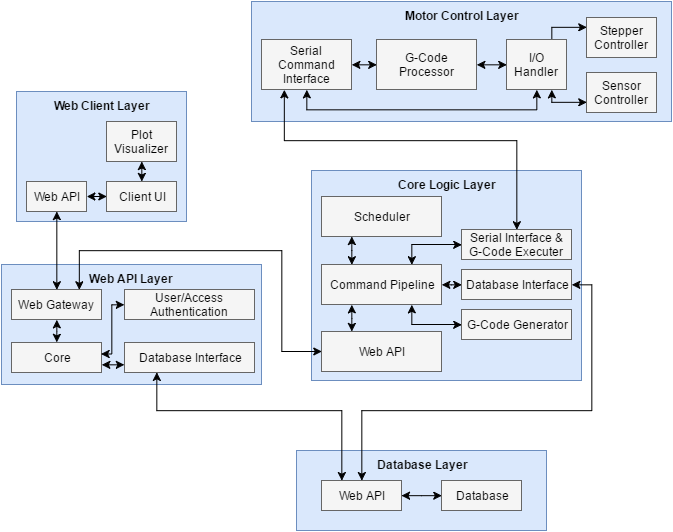
\includegraphics[width=\textwidth]{images/data_flow}
 \caption{A simple data flow diagram}
\end{figure}
